\subsection{Number representations}
\label{RSA_representation}

This section will be mainly dedicated to the different ways to represent 
numbers \textit{i.e.} integers or relative numbers. Plan id the following:
\begin{itemize}
	\item  Classical $b$-arry representations
	\item  Some binary representations
	\item  Non adjacent representations
\end{itemize}
AIM: Change the representation of a an integers or relative numbers for a new one.
What will be obtained might be a less simple, or might requires  more amount of digits but will be but richer in term of algebraic/computational proprieties(s).\\

\noindent
	\begin{mydef}{Canonical vs Non-Canonical representation}
		\begin{itemize}
			\item 'canonical' is used to indicate a standard way to represent a 
			mathematical object under the form of a mathematical expression.
    		This a particular convention that was accepted as standard among 
    		an important number of possible conventions. 
			\item 'non-canonical' by opposition means that the convention used to 
			to represent a mathematical object under the form of a mathematical 
			expression is not he standard one, therefore this expression is 
			meaningless unless convention to which it is referring is specified.
		\end{itemize}
    \end{mydef}		

Example:\\
In geometry, the canonical way to represent objects is referring to a Cartesian 
coordinate system system and no-one wonder what type of mathematical object 
represent the following expression $(x-h)^2+(y-k)^2= \rho^2$, 
(circle centered on $(h,k)$ and of radius $|\rho|$).
\newpage
\subsubsection{Mathematical notation}
Two way to interpret Euclidean division: \\

\begin{mydef}{Euclidean division:} \\
	Given $a,b $ positive integers there exist a unique couple of integers $ (q,r)$ \\
	such that decompose uniquely $a$ in the famous Euclidean form.\\
	\textit{i.e.} Given $a,b \in \mathbb{N}$ $\exists! (q,r) \in \mathbb{N}^2$, such that:
	\begin{center}
			$a = b \times q + r$ with $0\leq r <b$\\
	\end{center}
\end{mydef}		 
		As a consequence each number, can be decomposed the following way:\\
		$n = 2^k \times b  + r$ with $0 \leq r <2^{k-1}$. \\
		$n = 2^k \times b + r$ with $-2^{k-1}<r \leq 2^{k-1}$ \\\\
		The first equality is the canonical one, it allows representation in any $b$-basis with positive digits, whereas the second one, not canonical, enable representations in any binary basis with positive and negative digits but with 
		smaller absolute values -Useful for ECC, RSA with NAF exponent-.\\\\
		Iterating the division process on $a$ from the highest power of $b$ to 0, a link is naturally created between polynomial in $b$ and representation in basis $b$.\\\\
\textbf{Possible properties of $b$-basis representations}\\
* position relativity: representation in which the localization of a digit matters\\
* completeness for $\mathbb{S}$: each element of a set of number $\mathbb{S}$ can be represented\\
* uniqueness for $\mathbb{S}$: each element of $\mathbb{S}$ admits only one representative.\\
* homogeneity: representation in which all operations are performed in the same way.\\
* optimality: representation in which a propriety is minimized -Length, Hamming weight, many others-
among a larger family of representation.

Remarks:\\
* For positional representation system:
the basis is always written the same manner, $10$, consequence of link between $b$-arry representation/polynomial expansion of variable $b$:\\
$ 10 = 10_{10} $, $ 2 = 10_{2} $, $ b = 10_{b} $, $ -b = 10_{-b} $ \\
* Interesting properties are the span and shape of $\mathbb{S}$:\\
is this including negative number? is this a perfect, quite, strongly not, symmetrical span?\\
* In the following section, we always have $a \in \mathbb{S}$

Notation: \\
* $b \in \mathbb{N}^*$, basis will be $b$ or $-b$ \\
* $ \mathcal{D} $ is the digit space.\\
* $t$ number of bits of the considered architecture

\subsubsection{Classical $b$-arry representations}
Here are approached some classical general representations.

\begin{itemize}
	\item Unary notation: representation with $b=1$, \textit{aka} 'Peano Unary system'.\\
		Simplest way to represent integers numbers...\\
		For that representation to include $0$ we impose digit space to admits two elements\\
		$/!\backslash$ Formal -but non consistent with the general one- scripture
		\begin{small}
			\begin{center}	
		$ a_{1} = \sum \limits_{i=0}^{t-1} a_i$ and $\forall i, a_i \in \mathcal{D} =\{0,1\}$ 	
			\end{center}
		\end{small}
		* completeness for $\mathbb{S} = \llbracket 0, t \rrbracket$ \\
		* no uniqueness neither a positional system\\
		* the value 0 can only be implicitly represented by an empty digit string\\
		* addition is in fact concatenation, homogeneous\\
		
	\item $b$-arry notation: general canonical representation in base $b$, for $b \in \mathbb{N} \backslash \{0,1\} $ :\\	
		starting from the least significant digit, number is obtained via a polynomial in $b$ which coefficients are the digits of the number representative.
		\begin{small}
			\begin{center}	
				$ a_{b} = \sum \limits_{i=0}^{t-1} a_i \times b^i$ 
				and $\forall i, a_i \in	\mathcal{D} = \{0, ..., b-1\}$		
			\end{center}
		\end{small}	
		% A = (b-1) * sum b^i,i=0,t-1 = (b-1) * B, and 
		% B = (b^t-1)/(b-1)
		* unique representation for $\mathbb{S} =\llbracket 0, b^{t}-1\rrbracket$\\
		* homogeneity

	\item Signed $b$-arry notation: representation in base $b \in \mathbb{N} \backslash \{0,1\} $, \textit{aka} 'Sign and Magnitude  in base $b$'
		\begin{small}
			\begin{center}	
					$ a_{b,signed} = a_t \sum \limits_{i=0}^{t-1} a_i \times b^i$ and $\forall i, 
					a_i \in \mathcal{D} = \{0, ..., b-1\}$ 		
			\end{center}
		\end{small}	
		% from previous one
		* completeness for  $\mathbb{S}=\llbracket 1-b^{t-1}, b^{t-1}-1\rrbracket$ \\
		* non unique representation + 0 and -0\\
		* non homogeneous system ! \\
		* Simple to implement \\  
		* Symmetrical span
			
	\item Nega $b$-arry notation: canonical representation in base $-b$ 
		for $b \in \mathbb{N} \backslash \{0,1\} $ : 
		\begin{small}
			\begin{center}	
					$ a_{-b} = \sum \limits_{i=0}^{t-1} a_i \times (-b)^i$ 
					and $\forall i, a_i \in \mathcal{D}=\{0, .., b-1\}$ 		
			\end{center}
		\end{small}	
		% AM = (b-1) * sum (-b)^i, i=0,t-1   and i \in 2N = (b-1) * BM
		% BM = 		   sum (-b)^i, i=0,t-2   and i \in 2N
		% BM = 		   sum   b^(2i), i=0, t/2-1 = (b^t-1)/(b^2-1)
		% AM = (b-1) * (b^t-1)/(b^2-1)
		%
		% Bm =         sum (-b)^i, i=0,t-1   and i \in 2N+1
		% Bm = 		   sum (-b)^i, i=1,t-1   and i \in 2N+1
		% Bm =    -b * sum b^(2i), i=0, t/2-1
		% Am =    -b * (b-1) * (b^t-1)(b^2-1)
		%
		%$ -b \frac{b^t-1}{b+1}, \frac{b^t-1}{b+1}$	
		* completeness for a $\mathbb{S} = \llbracket -b \frac{b^t-1}{b+1}, \frac{b^t-1}{b+1}\rrbracket $ \\
		* completeness for $\mathbb{S}$ without bit sign ! \\
		* uniqueness for $\mathbb{S}$ \\
		* although arithmetic operations are more complicated, homogeneity of operations ! \\
		* $/!\backslash \hspace{1mm} \mathbb{S}$ not centered on 0, strongly asymmetrical span $\hspace{1mm} /!\backslash$

	\item  One's complement in base $b$ 
		\begin{small}
			\begin{center}	
					$ a_{b,1*} = (b^{t}-1)_b-a_b$ 
					% a = (b^t-1) - a_{b,1*}	
			\end{center}
		\end{small}	
		* except MSB, each bit is a power of $b$
	\item  Two's complement in base $b$ 
		\begin{small}
			\begin{center}	
					$ a_{b,2*} = b^{t}_b-a_b$ 				
					% a = b^t - a_{b,2*}
			\end{center}
		\end{small}	
		* except MSB, each bit is a power of $b$, except for the most significant bit,\\
		whose weight is the negative of the corresponding power of $b$.
\end{itemize}

\subsubsection{Some binary representations}
	\begin{itemize}	
		\item  Binary notation: canonical representation base 2:
		\begin{small}
			\begin{center}	
					$  a_{2}  =  \sum \limits_{i=0}^{t-1} a_i \times 2^i$ 
					and $\forall i, a_i \in \mathcal{D}= \{0,1\}$		
			\end{center}
		\end{small}	
			* Homogeneity\\
			* Complete for $\mathbb{N}$\\
			* Uniqueness for $\mathbb{N}$\\

		\item Signed binary: canonical representation in base $2$, \textit{aka} 'Sign and Magnitude in base $2$':
		\begin{small}
			\begin{center}	
					$  a_{2, signed} = {-1}^{a_{t-1}} \sum \limits_{i=0}^{t-2} a_i \times (2)^i$ 
					and $\forall i, a_i \in \mathcal{D}=\{ 0, 1\}$ 		
			\end{center}
		\end{small}
 		+ Simple to implement. \\ 
		+ Useful for floating point representation.  \\  
		- Sign bit independent of magnitude \\ 
		- can be  both + 0 and -0  (Makes math hard to do). \\  
		
		\item  One's complement canonical representation	
			\begin{center}	
				\begin{small}	
					$ a_{1*} = (2^{t}-1)_2-a_2 =\overline{ a_{2} }$,			
				\end{small}	
			\end{center}
			Except the MSB, each bit is a power of $2$\\
			The MSB is seen as the negative of $(2^{t}-1)$.\\
			And with a written as $ a_{1*} = \{a_{t-1}, a_{t-2}, ..., a_{1}, a_{0}  \} $ 
			\begin{center}	
				\begin{small}	
					% a = (b^t-1) - a_{b,1*}	

					$ a = - a_{t-1} (2^{t}-1) + \sum \limits_{i=0}^{t-2} a_i 2^{i}$
				\end{small}	
			\end{center}
			* completeness for $\mathbb{S}=\llbracket 1-b^{t-1}, b^{t-1}-1 \rrbracket$ \\
			* non uniqueness: two zeros $a_i=0$ and $a_i=1$\\
			* Feature: +0 and -0 return TRUE when tested for zero, FALSE when tested for non-zero. 

		\item  Two's complement canonical representation
			\begin{center}	
			If $a \geq 0$:
				\begin{small}	
					$ a_{2*} = a_2 $
				\end{small}	
			If $a \leq 0$:				
				\begin{small}	
					$ a_{2*} = 2^{t}_2-a_2 = \overline{ a_{2_{Signed}} }+1 $
				\end{small}					
			\end{center}
			Except the MSB, each bit is a power of $2$\\
			The MSB is seen as the negative of the corresponding power of $2$.\\
			And with a written as $ a_{2*} = \{a_{t-1}, a_{t-2}, ..., a_{1}, a_{0}  \} $ 
			\begin{center}	
				\begin{small}	
					$ a = - a_{t-1} 2^{t} + \sum \limits_{i=0}^{t-2} a_i 2^{i}$
				\end{small}	
			\end{center}
			* completeness for $\mathbb{S}=\llbracket -b^{t-1}, b^{t-1}-1 \rrbracket$ \\
			* homogeneity \\
			* there is one zero only. \\
			* multiplying 2's complement operands takes just about same amount of hardware as multiplying unsigned operand\\

		\item Nega binary: canonical representation in base $-2$: \\ 
		\begin{small}
			\begin{center}	
					$  a_{-2} =  \sum \limits_{i=0}^{t-1} a_i \times (-2)^i$ 
					and $\forall i, a_i \in \mathcal{D}=\{-1, 0\}$ 		
			\end{center}
		\end{small}
			* completeness for $\mathbb{S} \subset  \mathbb{Z} $ \\
			* $/!\backslash \mathbb{S}$ not centered on 0, strongly asymmetrical span$/!\backslash$
			* basic routines requires some efforts.\\

	\item Binary Signed Digit representation:\\
			Here is relaxed on condition on the digit of the representation, leading to non canonical representation.
			Here they have value in $\{-1, 0 , 1\}$, but the formal decomposition remain the same:
			\begin{center}
				\begin{small}
							$ a_{-1, 0 , 1} = \sum \limits_{i=0}^{t-1} a_i \times 2^i$  with $a_i \in \mathcal{D} =\{ -1,0,1\}$ \\
				\end{small}
			\end{center}
			The consequence it that number are not uniquely decompose: 	this is not canonical. 	\\
			On the other hand this additional degree of liberty allow to choose between	decompositions available.	

	\item Canonical Binary Signed Digit representation: \textit{aka} 'Binary-NAF'\\
			And precisely, without ambiguity, its name is '2-width Binary NAF'
\footnote{the width refers to the number among which only one will be allowed to be a non zero.}\\
			Here is relaxed on condition on the digit of the representation, leading to non canonical representation.
			Here they have value in $\{-1, 0 , 1\}$, but if the formal decomposition remain the same, one additional condition
			namely 'no adjacent 1' lead to one representation.
			\begin{center}
				\begin{small}
					$ a_{2-NAF} = \sum \limits_{i=0}^{t-1} a_i \times 2^i$  with $a_i \in \mathcal{D} =\{ -1,0,1\}$ \\
		    	 $\forall i \in \llbracket 0,t-1 \rrbracket,   a_i \times a_{i+1} =0$
				\end{small}			
			\end{center}	

		\item Binary Alternating Greedy expansion	
		this is a signed binary expansion, with the property that consecutive
		non zero digit -even if separated by some 0- are opposed.
		useful in several left-to-right algorihms

		\item Zeckendorf representation:\\
		A number can be decomposed in a unique way as a sum of Fibonnaci numbers,
		in which there is no two consecutive Fibonnaci number used.
		%* x^{F_n} can be computed with one initial squarring and only multiplication\\
		There exist a signed digit Zeckendorf representation.\\
		% http://www-pequan.lip6.fr/~bajard/GTArithIM/TRANSPARENTS/corps_finis/RAIM-Meloni.pdf
		$31 = {1010010}_F = F_8 + F_6 + F_3$
		\end{itemize}



		\subsubsection{Basic in geometry of numbers}

Recall:  finite field definition

The two following definitions are the start-point of a mathematical theory 
called  Algebraic Theory of Number, also-known-as 'geometry of numbers'.\\
\begin{mydef}{Algebraic number, algebraic integer}
    \begin{itemize}
	    \item[] $\overline{\mathbb{Z}}:= \{x\in \mathbb{C}/\exists P$
	    unitary,  $P\in \mathbb{Z}[X]^{\ast} / P(x)=0 \}$, 
	    ring of algebraic integers
	    \item[] $\overline{\mathbb{Q}}:= \{x\in \mathbb{C}/\exists P$ 
        $\in \mathbb{Z}[X]^{\ast} / P(x)=0 \}$, field of algebraic numbers 
    \end{itemize}

$\theta \in \overline{\mathbb{Q}}$ it is the root of many 
$P \in \mathbb{Z}[X]^{\ast}$, among them $P$ can be chosen irreducible, then
the degree of $P$, $d$ is called algebraic degree of $\theta$. We define 
\begin{center}
$\mathbb{Q}[\theta] := \{ x \in \mathbb{C} / \exists P\in \mathbb{Z}[X]$ and $x=P(\theta)$ \}
\end{center}

This  is a $\mathbb{Q}$-vector space 
of dimension $d$, a basis is $ \{ 1, \theta, \theta^2, \hdots,  \theta^{d-1}\}$\\
\end{mydef}
\begin{mydef}{'ring of integers an algebraic number field'}\\
Let $\mathbb{K}$ be a field of algebraic number 
$\textit{i.e.} \mathbb{K} = \mathbb{Q}[\theta]$.

 a ring can be defined, 
$\mathcal{O}_\mathbb{K} =  \overline{\mathbb{Z}} \cap \mathbb{K}$. 
Note that the field of fraction of the ring $\mathcal{O}_\mathbb{K}$ is $\mathbb{K}$.\\
\end{mydef}

\begin{myprop}{Quadratic field}\\
For $d=2, \mathbb{Q}[\theta]$ is snoted sliglty differently;
$\mathbb{Q}[\theta]=$
	\begin{center}
		$\mathbb{Q}[\sqrt{\theta}] := \{ x \in \mathbb{C} / x=a+b \times \theta$ with
$ a,b \in \mathbb{N} \}$
	\end{center}


and is named a quadratic field, according to the sign of $\Delta_P$, we be talked about 
'Imaginary quadratic field' ou 'Real' quadratic field'.


\end{myprop}

\begin{mythm}{'of classical imaginary quadratic field'}\\
Let be $\mathbb{Q}[\sqrt{d}]$ for some $d \in \mathbb{Z}$, 
square free additionally let's assume that $d<0$, 
then can explicit $\mathcal{O}_\mathbb{K} $:
	\begin{center} 
		$\mathcal{O}_\mathbb{K} = \mathbb{Z}[\alpha] $
		with $\alpha = \sqrt{d}$ if $d  = 2,3 \mod 4$ and 
		$\alpha = \frac{1+\sqrt{d}}{2}$ if $d  = 1 \mod 4$.\\
	\end{center}
\end{mythm}
%% https://en.wikipedia.org/wiki/Quadratic_field for name
Illustrations:
\begin{Large}
	\begin{table}[!h]
		\begin{center}
			\begin{tabular}{|c|c|c|c|c|c|}
				\hline 
$d$                       
    & $-1$ 
        &  $-2$
            & $-3$ 
                & $-7$ 
                    & $-11$ \\\hline  
$\mathbf{\theta}$ 
    & $1+\sqrt{-1}$ 
        &  $\sqrt{-2}$
            & $\frac{3+\sqrt{-3}}{2}$ 
                & $\frac{1+\sqrt{-7}}{2}$ 
                    & $\frac{1+\sqrt{-11}}{2}$ \\\hline 
$\mathbb{K}=\mathbf{\mathbb{Q}[\theta]}$ 
    & $\mathbb{Q}[1+\sqrt{-1}]$ 
        & $\mathbb{Q}[1+\sqrt{-1}]$
            & $\mathbb{Q}[\frac{1+\sqrt{-3}}{2}]$ 
                & $\mathbb{Q}[\frac{1+\sqrt{-7}}{2}]$ 
                    & $\mathbb{Q}[\frac{1+\sqrt{-11}}{2}]$ \\\hline
$\mathbf{\mathcal{O}_\mathbb{K}}=\mathbb{Z}[\alpha]$ 
    & $\mathbb{Z}[\sqrt{-1}]$ 
        & $\mathbb{Z}[\sqrt{-2}]$ 
            & $\mathbb{Z}[\frac{1+\sqrt{-3}}{2}]$ 
                & $\mathbb{Z}[\frac{1+\sqrt{-7}}{2}]$ 
                    & $\mathbb{Z}[\frac{1+\sqrt{-11}}{2}]$ \\\hline 
			\end{tabular}
		\end{center}
		\caption{$\theta$ chosen as non zero, non unit with $|\theta|>1$}
		\label{tab:esults}
	\end{table}
\end{Large}
 	\newpage
\subsubsection{Non Adjacent Forms}

\begin{center}			
	By opposition to unsigned digit notation, here 
	\textit{increase the size of the representation}\\ 
	can induce lower hamming weight and as a consequence a 
	\textit{faster exponentiation}.
\end{center}			

What's in the literature?
\cite{eurocrypt-1984-2410}

\cite{cciam-1997-joye} first part: present binary NAF and a natural converters. 
key paper.

\cite{pkc-2001-joye} introduce the compactification of a binary NAF representation,
leading a n-bit number to be represented as 2-NAF by n+1 bit \footnote{bit and not digit !} - key paper.

\cite{M2Thesis-Muir-2004} internship about NAF techniques and generalisation 
- NADS \& JDS- 

\cite{jofnt-2012-heuberger} provide a bit more  maths background for the complex NAF case


\cite{CanJMath-2008-blake} present complex NAF and give example for the following cases:
\begin{center}
$\tau =  1+\sqrt{-1}  $ \;\;
$\tau =  \sqrt{-2} $ \;\;
$\tau =  \frac{3+\sqrt{-3}}{2} $\;\;
$\tau =  \frac{1+\sqrt{-7}}{2} $\;\;
$\tau =  \frac{1+\sqrt{-11}}{2} $
\end{center}
\cite{latincrypt-2011-aranha} Was the fastest scalar multiplication for few months in 2011.






    \begin{figure}[!h]
        \centering
        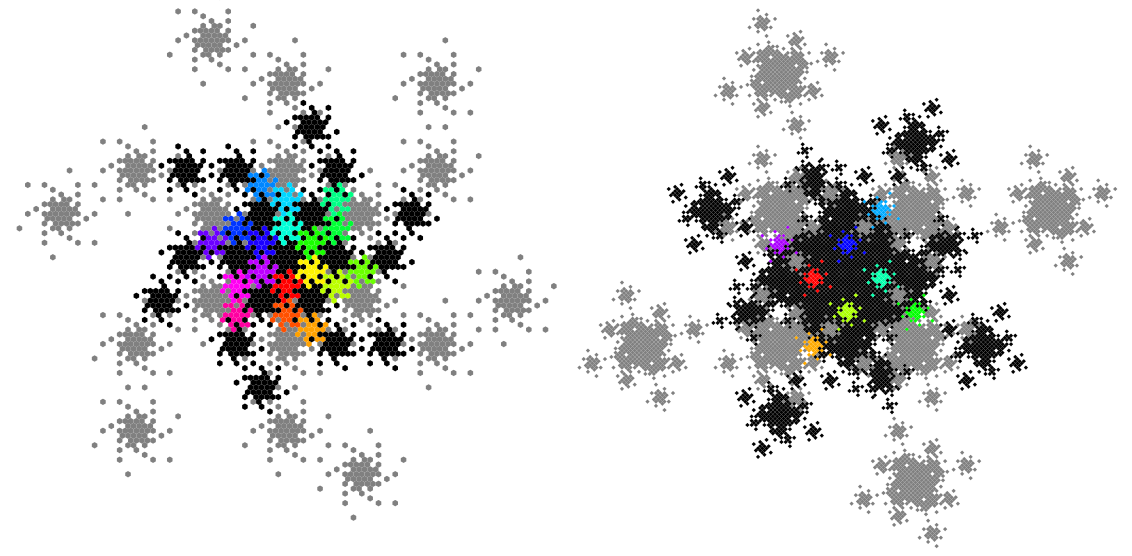
\includegraphics[width=15cm]{images/dessin.png}
\caption{3-NAF on the left, 4-NAF on the right - for different $\tau \in \mathbb{C}$}
    \end{figure}


					

\begin{itemize}	
	\item Binary Non Adjacent Form, 2-adic NAF form, 1-width 2-adic NAF form: \\
		Condition on the digits are relaxed allowing the
		coordinate $-1$ in addition to $0$ and $1$: 
		\begin{center}
			$\mathcal{D} =\{ -1,0,1\}$\\
		\end{center}
		\begin{center}
			\textbf{'NAF' meaningless   vs   ' 1-width 2-adic NAF' meaningful}\\
		'1-width' refers the maximum value in $\mathcal{D} $, \\
		'2-adic' refers to base's expansion, 2	
		\end{center}

	\begin{mythm}[Reitwiesner' 1960] 
		For a $a \in \mathbb{N} $, there exits a unique signed binary expansion noted, 
		$(a_i)_{0 \leq i \leq t-1 }$,
		 called the 1-width 2-adic NAF form of $a$
		such that:
		\begin{center}
		     $a =  \sum \limits_0^{t-1} a_1 \times 2^i$, with $a_i \in \mathcal{D} =\{ -1,0,1\}$ \\
		     $\forall i \in \llbracket 0,t-1 \rrbracket,   a_i \times a_{i+1} =0$
		\end{center}
        \begin{figure}[!h]
            \centering
        	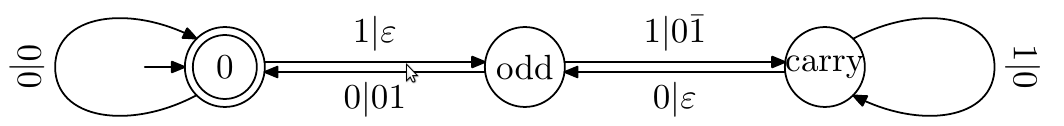
\includegraphics[width=15cm]{images/RtoL_unsignedbinary_to_2naf.png}
   		\end{figure}
	\end{mythm}


			\begin{center}
				\begin{tabular*}{10cm}{p{1.75cm}p{0.35cm}p{0.35cm}p{0.35cm}p{0.35cm}p{0.35cm}p{0.35cm}p{0.75cm}}		
     $ 23_{10} = \{$  &  0  &   1 &  0  &  1  &  1  &  1  &  $\}_2$\\	
     $ 23_{10} = \{$  &  0  &  1  &  1  &  0  &  0  & -1  &  $\}_2$\\
     $ 23_{10} = \{$  &  1  &  0  & -1  &  0  &  0  & -1  &  $\}_2$\\
				\end{tabular*}
			\end{center}

			Binary to binary 1-NAF definitions are not incompatible:
			\begin{center}
				\begin{tabularx}{10cm}
{p{1.5cm}p{0.35cm}p{0.35cm}p{0.35cm}p{0.35cm}p{0.35cm}p{0.35cm}p{0.75cm}}
$ 42_{10} = \{$  &  1  &   0 &  1  &  0  &  1  &  0  &  $\}_2$\\	
				\end{tabularx}
			\end{center}


    \begin{figure}[!h]
        \centering
        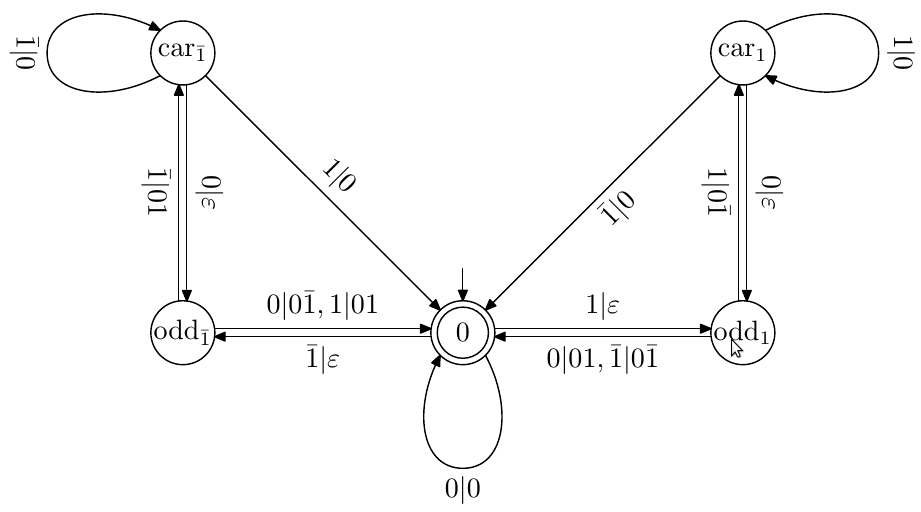
\includegraphics[width=15cm]{images/RtoL_allsignedbinary_to_2na0f.png}
		\caption{Visual proof for previous affirmation}
    \end{figure}

    \begin{mydef}{Optimality for a given digits space} :			
			An expansion of $a$  is said to be optimal, if it minimizes the weight
			among all the of $a$ with digits out of $\mathcal{D}$.\\
	\end{mydef}
		
	\begin{mythm}[Reitwiesner' 1960] 
			binary-NAF of integers is optimal among all expansion
			using the following digits $\mathcal{D} =\{ 0,\pm 1\}$.				
	\end{mythm}
			
		\underline{Theorems:} 
\begin{itemize}
\item 2-adic NAF representation have , at most, one digit longer than its a binary representation.
\item Each integer has a unique 2-adic NAF representation.
\end{itemize}

\textbf{1-width 2-adic NAF form: ECC vs RSA}
\begin{itemize}
\item[RSA case:] 'Square-and-Multiply' has to be changed to 'Square-and-Multiply-or-Divise'\\
and the value $x^{-1} \mod n$ shall be precomputed.\\ 
\item[ECC case:] 'Double-and-Add' algorithm should be changed to 'Double-and-Add-or-Substract' \\
and the value $-P $ should be precomputed.

But here is a trick : in many ECC implementation compute the opposite of a point 
is very easy: in this case: binary NAF applied to ECC saved a pre-computed value 
by comparison to RSA the same representation applied to RSA.
\end{itemize}





\newpage
	\item Extended Binary NAF or $k$-width 2-adic NAF, canonical representation\\
		extension of the 2-NAF: the base is still $\tau=2$,
		but the digit space is increased ...
			\begin{center}
$a =  \sum \limits_0^{t-1} a_I \times 2^i$,
with $a_i \in \mathcal{D} =\{ 0,\pm 1, \pm 3, .., \pm 2^{k-2}-1 \}$ \\
$\forall i \in \llbracket 0,t-1 \rrbracket,$
Among $k$ consecutive digits max one of them is non-zero\\
Each non zero digit is odd.
			\end{center}

%			width 	max digits 		formula
%2 			+/- 1  		2^(2-1)-1
%3 			+/- 3  		2^(3-1)-1
%4 			+/- 7  		2^(4-1)-1
%5 			+/- 15  	2^(5-1)-1

		\underline{Theorems:} 
\begin{itemize}
\item $k$-width 2-adic NAF representation, 
at most, one digit longer than its binary representation.
\item Each integer has a unique $k$-width 2-adic NAF.
\end{itemize}

		\underline{Theorem:} Avanzi, Muir \& Stinson' 2004\\
		With $\tau = 2$, $k \geq 2$, extended binary NAF of each integer 
		is optimal for $\mathcal{D} =\{ 0,\pm 1, \pm 3, .., \pm 2^{k-2} \}$.	
	



\end{itemize}						
		\underline{General converter}
			The following routine returns the $\omega$-width binary NAF of a binary 
			
			\begin{algorithm}[h]
				\KwIn{$n \in \mathbb{N}$}
				\KwOut{$n \in \mathbb{N}$}										 
				\If{ $n=0 \mod 2$  }{ \Return{$ n/2 $}	} 					 
				$r \leftarrow -2^{k-1}<r \leq 2^{k-1}$ 
				with $n = b \times 2^k + r$. \;					
				\Return{$n\leftarrow (n-r)/2^{\omega}$  }									
				\caption{function $f_\omega(n)$}
			\end{algorithm}	
			\begin{algorithm}[h]
				\KwIn{$n \in \mathbb{N}$}
				\KwOut{$n \in \mathbb{N}$}										 
				\If{ $n=0 \mod 2$  }{ \Return{$ 0 $} } 
				$r \leftarrow -2^{k-1}<r \leq 2^{k-1}$ with $n = b \times 2^k + r$. \;	
				$0^{k-1}r$			 				
				\caption{function $g_\omega(n)$}
			\end{algorithm}					
			\begin{algorithm}[h]
				\KwIn{$n \in \mathbb{N}$}
				\KwOut{a string of digits}	
				$\alpha \leftarrow$ ''												 
				\While{ $n \neq 0$ }{
				$\alpha \leftarrow g_{\omega}(n)\,||\,\alpha $\;
				$ n \leftarrow f_{\omega}(n)$ 
					} 
				\Return{$ \alpha $}												 				
				\caption{Binary to $\omega$NAF converter}
			\end{algorithm}	

	
\underline{examples}\\
$g(2)(n)$ will take the values: $     0, 01, 01, 01$\\
$f(2)(n)$ will take the values: $42, 21,  5,  1, 0$\\
then the 2NAF form of 42 is $0101010_2$ meaning $42_{10}= 2^5+2^3+2^1$.
		
$g(3)(n)$ will take the values: $ 0,  00-3, 003$\\
$f(3)(n)$ will take the values: $42,  5,    1, 0$\\
then the 3NAF form of 42 is $300-30_2$ meaning $42_{10}= 3 \times2^4 -3 \times 2^1$.		

$g(4)(n)$ will take the values: $ 0,  00-3, 003$\\
$f(4)(n)$ will take the values: $42, 21, 3, 0$	\\
then the 4NAF form of 42 is $300-30_2$ meaning $42_{10}= 3 \times2^4 -3 \times 2^1$.

$g(5)(n)$ will take the values: $ 0, 0000-11, 0002$\\
$f(5)(n)$ will take the values: $42, 21, 1, 0$\\
then the 5NAF form of 42 is $000010000-10_2$ meaning $42_{10}= \times2^7 -11 \times 2^1$..
%	3 0 0 -3 0  = 3 * 2^4 + 0 * 2^3 + 0 * 2^2 + 3 * 2^1 + 0 * 2^0 = 42.
%
%w = 3, then f3(13) = 2 and g3(13) = 00-3.

\newpage
\textbf{$k$-width 2-adic NAF form: ECC vs RSA} ... example with $k=3$
\begin{itemize}
\item[RSA case:] 'Square-and-Multiply' has to be changed to 'Square-and-Multiplyor-Divise'\\
and the values $\{ - 1, \pm 3 \} $ shall be precomputed.\\ 
\item[ECC case:] 'Double-and-Add' algorithm should be changed to
'Double-and-Add-or-Substract' \\
and only the value $3P $ should be precomputed, in the case of a curve 
giving cheap inversion.

	\item Real Non-Binary based NAF: Non-Binary NAF and Non-Binary $k$-NAF:\\
    Here simply the base $\tau$ is not two any more, but another prime.    

	\item Complex NAF and $k$-NAF form:\\
		This time is $\tau \in \mathbb{C}^\ast$ and is algebraic integer over
		$\mathbb{Z}$ of degree 2 
		\footnote{\textit{i.e} root of some $x^2-p \times x + q \in \mathbb{Z}$[x]}
		with $|\tau| > 1$ and $k \geq 2$
 
	\begin{mydef}
	 \textit{Zero \& local Voronoi Cells:}\\
		The Voronoi cell at origin is :
 		\begin{center}
 		$V :=\{ z \in \mathbb{C}: \forall y \in \mathbb{Z}^{\ast}[\tau],
 		\|z\|\leq \|z-y\| \} $
 		\end{center}
 		 		By definition the Voronoi Cell for the point $u \in \mathbb{Z}[\tau]$ 
 		corresponding to set $\mathbb{Z}[\tau]$ where $u$ is then called 
 		centre of $V_u$, or the lattice point corresponding to $V_u$, is such as:
 		\begin{center}
 		$V_u :=\{ z \in \mathbb{C}: \forall y \in \mathbb{Z}[\tau],
 		\|z-u\|\leq \|z-y\| \} $
 		\end{center}
	\end{mydef}

        \begin{figure}[!h]
          \centering
          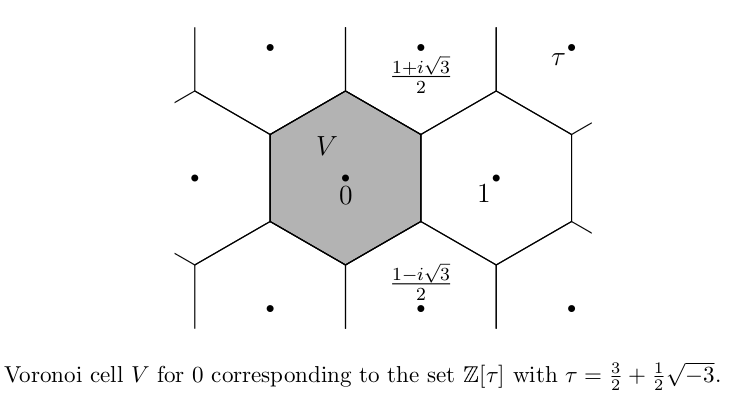
\includegraphics[width=15cm]{images/voronoi.png}
        \end{figure}
        Remark that the limit case given by equation of the definition
 		$ \|z\| = \|z-y\| $ share the plan in two via the bisection of 
 		segment $[zy]$ which fully make sense when $z$ is an extremal point.
        \newpage

        \raggedleft 
		... From now on $\mathcal{D}$ is assumed to be a 'Restricted Voronoi Cell' \\
		\raggedright		
	\begin{mydef} \textit{Restricted Voronoi Cell:}\\
        Previous definition was unclear about to which cell borders 
        -vertices + edges- belong to.
        Each edge is split in two equal part, defining three points of each of them,
        defining twice more points and portions of line than there was of vertices 
        and edges, then those elements are fairly shared (segment , points) 
        on each side of the origin.         
        This new cell is called 'Restrictive Voronoi Cell', and noted $\tilde{V}$
        \begin{figure}[!h]
          \centering
          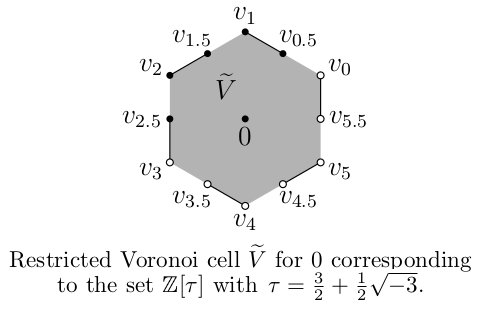
\includegraphics[width=10cm]{images/voronoi_restricted.png}
          \caption{     \textit{if $stuff \in V_u$ then its symmetrical don't}.}
        \end{figure}
    \end{mydef}
\raggedleft 

... From now on $\mathcal{D}$ is assumed to be a 'Reduced Residue Digit Set' \\
\raggedright
	\begin{mydef}{Reduced Residue Digit Set}\\
		For $\mathcal{N}(\tau^k) \leq 12$, we note 
		\begin{center}
		$R = \{x \in \mathcal{O}_\mathbb{K}$ such that $\tau \not\vert x \}$
		\end{center}
		The set $\mathcal{D} \subseteq \mathbb{Z}[\tau]$ is called 
		'reduced residue digit set modulo $\tau^k$', 
		if it consist of $0$ and exactly one representative for each 
		residue class of $R \mod \tau^k$ that is not divisible by $\tau$.
		
		More precisely:\\ 
		if a class contain a unit $u$ then: 
		$\mathcal{D} := \mathcal{D} \cup \{u\}$\\
		if a class do not contain a unit: 
		$\mathcal{D} := \mathcal{D} \cup \{u$ such that $ |u|\leq \mathcal{N}(\tau^k) \}$\\
	\end{mydef}
\vspace{5mm}


\textbf{Definition:} 
\textit{RDS $k$-Width $\tau$-adic Non Adjacent Form} 
or  
\textit{$k$-Width NADS:}
\\
Let's  $\mathbf{\eta}=(\eta_j)_{j} \subset \mathcal{D}^\mathbb{Z}$ .
The representation $ \eta $ is called $k$-Width $\tau$-adic Non Adjacent Form
if each factor $\eta_{j+k-1}...\eta_{j}$, \textit{i.e.} each block of length $k$
contains, at most, one non-zero digit.
\vspace{5mm}

\textbf{Theorem} 
\begin{center}
	Let's $k>2$, $\mathbb{K}=\mathbb{Q}[\tau]$ and  $\mathcal{D}$ 
	be a $k$-Width NADS and  \\
	we have $\forall x \in \mathcal{O}_\mathbb{K}, \; \exists ! $ 
	RDS $k$-Width $\tau$-adic NAF for $x$.
\end{center}

Remark: in certain cases the condition $k>2$ can be relaxed:

for $ \tau = \frac{3+\sqrt{-3}}{2}$, $k>1$\\
for $ \tau = \frac{1+\sqrt{-7}}{2}$, $k>1$\\
for $ \tau = \frac{1+\sqrt{-11}}{2}$, all $k$ \\

\newpage
\raggedleft 
... From now on element of $\mathcal{D}$ are assumed to be a
'Representatives of Minimal Norm' \\

\raggedright
	\begin{mydef}{Representative of Minimal Norm}\\
			Let $\tau$ be an algebraic integer, imaginary quadratic and let 
		$\eta \in \mathbb{Z}[\tau]$ be not divisible by $\tau$. \\
		Then if $\eta \in \tau^k \times \tilde{V}$ is called 
		'Representative of Minimal Norm'

        \begin{figure}[!h]
          \centering
          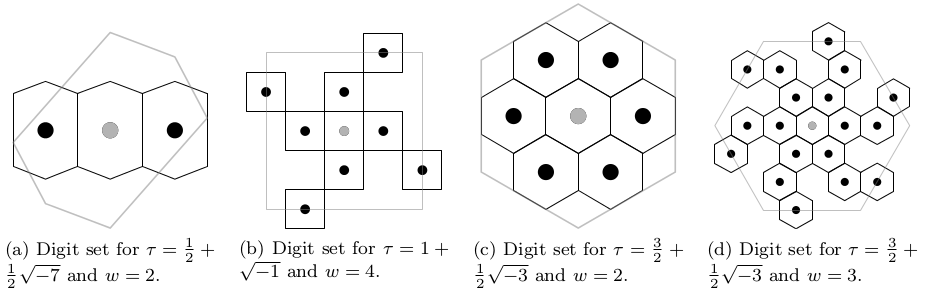
\includegraphics[width=18cm]{images/voronoi_save.png}
        \end{figure}
    \end{mydef}

\begin{itemize}
\item Minimal norm representatives digits set modulo  $\tau^k$ for several $\tau$ and $k$.
\item For each $\tau$, $V_\tau$ is drawn; the large cell is $\tau^k \times V$.
\item the situation c) verify the previous definition 
\end{itemize}
\vspace{3mm}

\raggedleft 
... From now on element of $\mathcal{D}$ are assumed to be a 'Minimal Norm Representative Digit Set' \\
\raggedright
		Definition - \textit{Minimal Norm Representative Digit Set:} \\
		Let $\tau$ be an algebraic integer, imaginary quadratic 
		and let $\mathcal{D}$ be reduced residue digit set modulo $\tau^k$
		consisting of representative of minimal norm if its residue class,
		then $\mathcal{D}$ is called 'Minimal Norm Representative Digit Set'.\\
\vspace{3mm}

.... And here it is:
\vspace{3mm}

		\textbf{Definition} \textit{$k$-Width $\tau$-adic Non Adjacent Form:} \\
Let's  $\mathbf{\eta}=(\eta_j)_{j} \in \mathcal{D}^\mathbb{Z}$ .
The representation $ \eta $ is called $k$-Width $\tau$-adic Non Adjacent Form

if each factor $\eta_{j+k-1}...\eta_{j}$, \textit{i.e.} each block of length $k$
contains, at most, one non-zero digit.\\
\vspace{3mm}

\begin{mythm} 
	For each lattice point  $x \in \mathbb{Z}[\tau]$ 
	and  $\mathcal{D}$ be a $k$-Width MNR\\
	we have $\forall x \in \mathbb{Z}[\tau], \; \exists ! $ 
	MNR $k$-Width $\tau$-adic NAF for $x	$.
\end{mythm}

\vspace{5mm}		
		\underline{Theorem:} Avanzi, Muir \& Stinson' 2004\\
		In the complex case with $\tau = 2$, $k \in \{2, 3\}$,
		the $\tau^k$-NAF  is optimal.

		\underline{Theorem:} Heuberger' 2010\\
		In the complex case with $k \in \{4,5,6\}$,
		the $\tau^k$-NAF is NOT optimal.


		\underline{Theorem:} Krenn' 2011\\
		In the following cases:
		$k \geq 4$, $\|p\| \geq 3$ or $k = 3  $, $\|p\| \geq 5$ 

		In the complex case with $k \in \{4,5,6\}$,
		the $\tau^k$-NAF is optimal.

	\end{itemize}
		\underline{Example:} binary to binary NAF conversion\\
			 An intuitive algorithm without pretending to any efficiency is
			'starting form LSB if two consecutive non zeros digit are meet
			change the smallest for -1 and propagate the change. 
			
			The process will always terminates with a valid NAF representation of $n$,
			process start and begin at position entirely determined	by ${n_2}$, 
			noting that the it is a fully reversible process.
			   			     
\underline{Important remark:}
Strictly speaking the difference between a Square \&  Multiply and a $2^3$-arry 
method is only a change in the representation from base 2 to base $2^3$, 
and using the same exponentiation algorithm.

		 
\newpage		
\subsubsection{Illustration of complex NAF:}



This section is dedicated to give an basically meaningful example 
of use of complex NAF, the given example is for primary field, then 


Let assume $ P $ is a point on the hereafter defined curve$ \mathbb{E} $,
and let $n$ and integer and $n P$ to be computed.

\begin{center}
$\mathbb{E}({\mathbb{F}_5}^m):  y^2 = x^3 -x  +2$ over $ {\mathbb{F}_5}^m $
\end{center}

How many point on the curves $\mathbb{E}({\mathbb{F}_5}^m)$? depending on $m$\\
How many point on the curves $\mathbb{E}({\mathbb{F}_5})$? let's see
		

%\noindent
%\begin{minipage}{\textwidth}[t][0.5 \textheight][t]

%\end{minipage}

	\begin{figure}[htbp]
		\begin{minipage}[c]{.70\linewidth}
			\begin{center}
				\begin{tabular}{|p{15mm}|p{15mm}|p{15mm}|p{15mm}|}
					\hline \rowcolor[rgb]{.8,.8,.8} 
					$x$ & $x^3 -x  +2$ & $y$ & $ y^2$\\
					\hline
					$ 0 $ & $ 2 $ & $ 0 $ & $ 0 $\\
					\hline
					$ 1 $ & $ 2 $ & $ 1 $ & $ \mathbf{1} $\\
					\hline
					$ 2 $ & $ 3 $ & $ 2 $ & $ 4 $\\
					\hline
					$ 3 $ & $ \mathbf{1} $ & $ 3 $ & $ 4 $\\
					\hline
					$ 4 $ & $ 2 $ & $ 4 $ & $ \mathbf{1} $\\
					\hline
				\end{tabular}						
			\end{center}		
		\end{minipage}
		\hfill
		\begin{minipage}[c]{.30\linewidth}	
			$\mathcal{O}$\\
			$(3, \pm 1)$\\
			$(3, \pm 4)$\\
		\end{minipage}
		\caption{$\mathbb{E}({\mathbb{F}_5}) = \{ \mathcal{O} ; (3, \pm 1) \}$}
	\end{figure}
Then we define the Frobenius isomorphism as usual:
\begin{center}
 $ \sigma=\left\{ 
 \begin{array}{ll}  
 \mathbb{E}  \longrightarrow \mathbb{E} \\
  (x,y) \mapsto (x^5,y^5)
 \end{array} \right.$
\end{center} 

Then according to REFERENCE, Frobenius morphism has for characteristic polynomial:
$\Phi^2 -a \times \Phi +q$ where $a = q+1 - \mathbb{E}({\mathbb{F}_q}) $ and here $q=5$
That is to say $\Phi^2 -3 \times \Phi + 5$

The previous decomposition lead us to use representation in $\mathbb{Q}[\sqrt{-11}]$

Avoid weakness on $\mathbb{E}({\mathbb{F}_5}^m)$, $m$ should not be stupidly chosen.

Then $\omega$-width $\tau$-adic NADS is prepared, with $\tau = \frac{1+\sqrt{-11}}{2}$,
According to the value of $\omega$, the digit space of $ \mathbb{D} $ is defined 
and $\omega$-width $\tau$-adic NADS conversion algorithm is defined.

\begin{enumerate}
\item Check that the considered representation exist
\item Convert $n$: compute $a+b \times \tau$ such that 
	$n \equiv a+b \times \tau \mod (\tau^m -1)$ 

	this trick has a name!\\
	since $(\tau^m -1) \times P =\mathcal{O}$, we have $n \times P = ( a+b \times \tau) P$

\item Convert $ a+b \times \tau$ to $\omega$-width $\tau$-adic NADS
\begin{center}
	$  a+b \times \tau  = \sum \limits_{i=0}^s c_i \tau^{k_i}$
\end{center}
\item for each $c \in \mathbb{D}$ pre-compute $Q_c = c \times  P$

\item Exponentiation is done trough a Horner scheme:\\
$(a+b  \tau) \times P  = 
\tau^{k_1}(\tau^{k_2-k_1} (... (\tau^{k_s-k_{s-1}}\times Q_{c_s} + Q_{c_{s-1}} )+ ... +)
+Q_{c_1})+Q_{c_0} $

\end{enumerate}
For binary fields, using normal basis, the cost of 'a Frobenius' is a shift



\subsection{Group representations}

\subsubsection{Chinese Theorem of Remainders:}
Elements of some finite fields $ \mathbb{Z}/{n \mathbb{Z}} $, 
where $n$ is a product of primes
\begin{itemize}
	\item Canonical representation in $ \mathbb{Z}/{n \mathbb{Z}} $,\\
	4 times slower tan CRT to achieve an RSA exponentiation.	
	
	\item Uses of Chinese theorem of remainders, 
	smaller number fastening the computations.
	Require a recombination step: Gauss, Garner, ...

	\noindent
	\textit{VS side channel cryptanalysis}\\
Because of the recombination step, that can be side channel analysed or even
perturbed, the CRT implementation bring also some potential weaknesses.
\end{itemize}

			\begin{algorithm}[h]
				\KwIn{$p, q, S_p, S_q, q^{-1}  \mod p, p^{-1}  \mod q$}
				\KwOut{$S = m^d \mod n$}	
				$S \leftarrow 
				S_p \times q \times (q^{-1} \mod p) +
				S_q \times p \times (p^{-1} \mod q) $\;	
				\Return{$ S $}												 				
				\caption{Gauss recombination}
			\end{algorithm}
			Remark: very natural but terribly slow as two modular inversions are required!
			\begin{algorithm}[h]
				\KwIn{$p, q, S_p, S_q, q^{-1}  \mod p$}
				\KwOut{$S = m^d \mod n$}	
				$t \leftarrow S_p-S_q$\;
				\If{ $t < 0$ }{ 
				$t \leftarrow t+p$\;
					} 
				$t^{'} \leftarrow t \times (q^{-1} \mod p)$	\;
				$S \leftarrow S_q + t^{'} \times q$\;	
				\Return{$ S $}												 				
				\caption{Unprotected Garner algorithm}
			\end{algorithm}
			
			\begin{algorithm}[h]
				\KwIn{$S_p, S_q, p, q, q^{-1}  \mod p$}
				\KwOut{$S = m^d \mod n$}	
				$t_0 \leftarrow S_p- S_q$\;
				$t_1 \leftarrow t_0 +p$\;
				\If{ $t_0 < 0$ }{ 
				$t \leftarrow t_1$\;
					}
				\If{ $t_0 > 0$ }{ 
				$t \leftarrow t_0$\;
					} 	 
				$t^{'} \leftarrow t \times (q^{-1} \mod p)$	\;
				$S \leftarrow S_q + t^{'} \times q$\;		
				\Return{$ S $}												 				
				\caption{Non conditional Garner algorithm}
			\end{algorithm}	
			
			\begin{algorithm}[h]
				\KwIn{$S_p, S_q, p, q, q^{-1}  \mod p$}
				\KwOut{$S = m^d \mod n$}	
				$t_0 \leftarrow S_p- S_q$\;
				$t_1 \leftarrow t_0 +p$\;
				\If{ $t_0 < 0$ }{ 
				$t \leftarrow t_1$\;
					}
				\If{ $t_0 > 0$ }{ 
				$t \leftarrow t_0$\;
					} 	
				$t^{'} \leftarrow t \times (q^{-1} \mod p)$	\;
				$S^{'} \leftarrow S_q + t^{'} \times (q+R)$\;
				$ S \leftarrow S^{'}  \mod  N$\;	
				\Return{$ S $}												 				
				\caption{Non conditional DPA-protected Garner algorithm}
			\end{algorithm}	






